\chapter{XML and Query Languages}

In this chapter, we introduce XML and two query languages: XPath
and XQuery, used in this study.


\section{XML}

XML~\cite{XML} is a standard data describing language used for representing
arbitrary data in a hierarchical structure. As introduced, XML
documents are increasing dramatically in size over time. Large XML documents in
this thesis refer to XML documents whose sizes are greater than 1 gigabytes.

Each XML document corresponds to a logical XML tree (or simply tree) that
contains one or more elements.  There are several types of elements in the tree
of an XML document. In this study, we focus on the following three element
types.

\begin{itemize}
	\item Element node \\
	An element node is parsed from a pair of tags, a start tag and a end tag, and
	are used to represent the structure of an XML tree. All element nodes are
	ordered as their corresponding tags appear in the XML document.
	\item Content node \\
	A content node (also called value node) represents the value of a element node.
	\item Attribute node \\
	An attributes node is used to associate name-value pairs inside a start tag of
	an element node for describing properties of the element node.
\end{itemize}

% Nodes are ordered.

Now, we give an example to show what these nodes are. Given the following
XML text string.\\

\hspace{10ex}\texttt{<A>}

\hspace{14ex}\texttt{<B AT1="VAL1">TXT1</B>}

\hspace{14ex}\texttt{<D>}

\hspace{18ex}\texttt{<E AT2="VAL2"></E>}

\hspace{18ex}\texttt{<F>}

\hspace{22ex}\texttt{<G>}

\hspace{26ex}\texttt{<I></I>}

\hspace{22ex}\texttt{</G>}

\hspace{22ex}\texttt{<H>TXT2</H>}

\hspace{18ex}\texttt{</F>}

\hspace{18ex}\texttt{<J></J>}

\hspace{14ex}\texttt{</D>}

\hspace{14ex}\texttt{<K>}

\hspace{18ex}\texttt{<L>TXT3</L>}

\hspace{14ex}\texttt{</K>}

\hspace{10ex}\texttt{</A>}\\

We can create an XML tree as shown in Figure~\ref{fig:relationships} (The
example of three element types are shown on left-bottom corner). For example,
the node B is an element node. There two nodes below B and are connected to it.
The left one  is an attribute node with the name `AT1' and the value `VAL1'. The
right  one is a value node with the string value `TXT1'.

\begin{figure}[t]
	\centering
	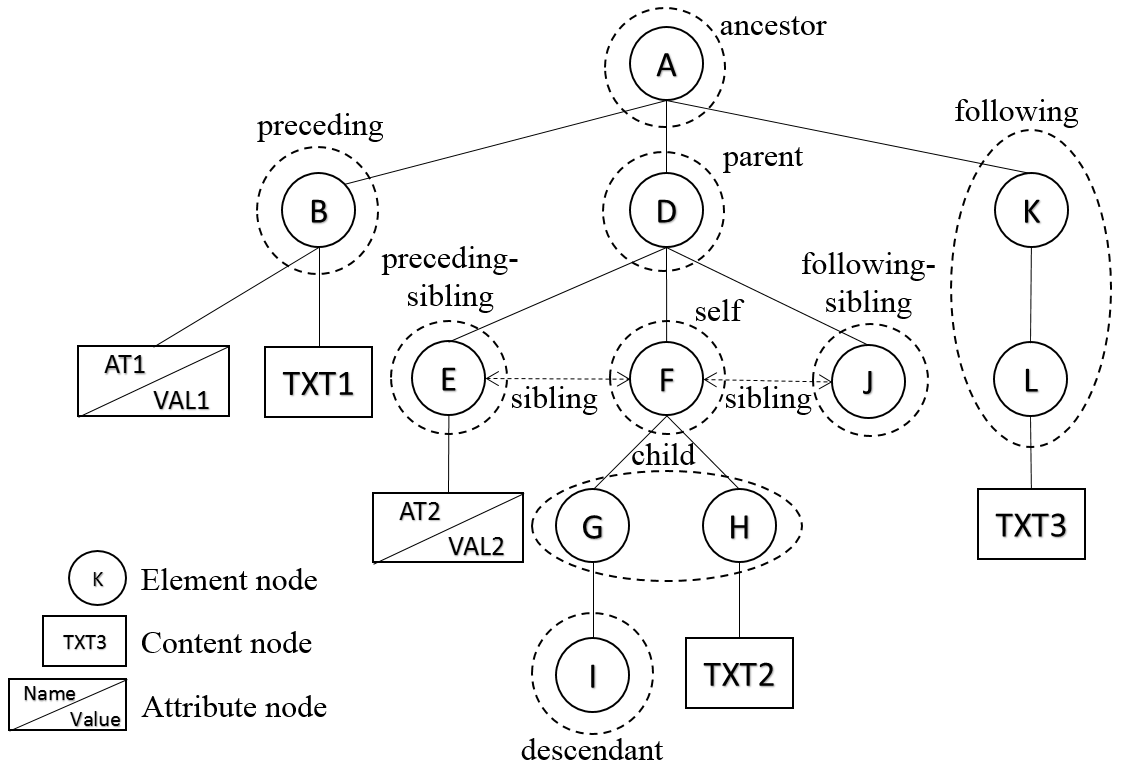
\includegraphics[width=1\linewidth]{figures/relationships}
	\caption{An example of node relationships.}
	\label{fig:relationships}
\end{figure}



\section{XPath Language}
\label{sec:xpath}

\subsection{Definition of XPath}

XPath is an XML query language used for selecting parts of an XML
document~\cite{xpath}. XPath queries are represented in path expressions. Each
path expression contains one or more \emph{location steps} or simply
\emph{stpes}. In this study, each step consists of an \emph{axis}, a \emph{name
test}, and at most one \emph{predicate}.

An axis defines the relationships of the current node and the target nodes.
There are 12 axes supported in this study, including  \texttt{child},
\texttt{descendant}, \texttt{parent}, \texttt{ancestor},
\texttt{descendant-or-self}, \texttt{ancestor-or-self}, \texttt{following},
\texttt{following-sibling}, \texttt{preceding}, \texttt{ preceding-sibling}  and
\texttt{attribute}. Note that \texttt{attribute} is different from the the other
axes. Because it selects only attribute nodes, while the other axes select only
element nodes. Content nodes can be selected by using function \texttt{text()}.
Figure~\ref{fig:relationships} uses node F as the current node to demonstrate
these axes. In the figure, F has a parent D, two siblings: E  on the left side
as a preceding-sibling and I on the right side as a following sibling, two
children: G and H, one descendant I, one preceding B, and two followings: nodes
K and L.

A name test is used for selecting nodes. If the name of a tag in an XML document
is equal to the name test, the node is selected. XPath also defines a wilecard  `*'
that matches with any name.

A predicate written between ``\verb|[|'' and ``\verb|]|'' describes additional
conditions to filter the matched nodes by using a path.

For example, given a query
``\verb|/descentdant::F[following-sibling::J]/child::H|'', this XPath query has
two steps where \verb|descendant| and \verb|child| are the axes, \verb|F| and
\verb|H| are the name tests, and a predicate \verb|child::H| is attached to the
second step.

\subsection{Evaluting XPath query}


\begin{figure}[!t]
	\centering\fbox{
		\begin{minipage}{.95\linewidth}
			\textit{Query} ::= `\texttt{/}' \textit{LocationPath}          \\
			\textit{LocationPath} ::= \textit{Step} $~|~$ \textit{Step} `\texttt{/}' \textit{LocationPath}          \\
			\textit{Step} ::= \textit{AxisName} `\texttt{::}' \textit{NameTest} \textit{Predicate}?          \\
			\textit{AxisName} ::= `\texttt{self}' $~|~$ `\texttt{child}' $~|~$ `\texttt{parent}'   $~|~$ `\texttt{descendant}'   $~|~$ `\texttt{ancestor}'          \\
			\phantom{\textit{AxisName} :}  `\texttt{descendant-or-self}' $~|~$ `\texttt{ancestor-or-self}'  $~|~$ `\texttt{following}'    \\
			\phantom{\textit{AxisName} :}        $~|~$ `\texttt{following-sibling}'  $~|~$ `\texttt{preceding}  $~|~$ `\texttt{preceding-sibling}'          \\
			\phantom{\textit{AxisName} :}        $~|~$ `\texttt{attribute}'   \\
			\textit{NameTest} ::= `\texttt{*}' $~|~$ \textit{string}	          \\
			\textit{Predicate} ::= `\texttt{[}' \textit{SimpleLocationPath} `\texttt{]}'          \\
			\textit{SimpleLocationPath} ::= \textit{SimpleStep} $~|~$ \textit{SimpleStep} `\texttt{/}' \textit{SimpleLocationPath}          \\
			\textit{SimpleStep} ::= \textit{AxisName} `\texttt{::}' \textit{NameTest}
		\end{minipage}
	}
	\caption{Grammars of XPath queries used for partial tree}
	\label{fig:grammar}
\end{figure}


When evaluating an XPath query, we start from the first step and evaluate each
location step in order. When meeting a predicate, we process it as a filter to
rule out unmatched nodes. Let us continue to use the query above to demonstrate.
This query first retrieves all the nodes with name \verb|F| in a XML document,
and then among their children it retrieves node \verb|H| with one or more
children with name \verb|J|. In other words, the result of the query is a set of
nodes \verb|H|, each of which has its parent \verb|F| and at least one sibling
\verb|G| on its right. The grammar of XPath used in this study for our novel
tree structure partial tree (See Chapter~\ref{ch:partialtree}) is listed in
Figure~\ref{fig:grammar}.


\section{XQuery}

XQuery is also a language for querying XML documents. It for XML is like SQL for
databases. It integrates with XPath language and an XPath query in an XQuery
expression returns exactly the same result as in XPath language. XQuery is more
expressive and powerful (also more complicated) than XPath.  Now, let use
consider the following expression as an example. In this study, we used XQuery
3.1~\cite{XQuery3_1}.

\begin{lstlisting}
for $x in doc("books.xml")/bookstore/book
return $x/title
\end{lstlisting}

This XQuery expression queries an XML document, namely ``books.xml''. It
evaluates an XPath query \texttt{/bookstor/book} over the document to select all
\texttt{book} of the root \texttt{bookstore} and returns the \texttt{title} of
the selected \texttt{book}.

\section{Summary}

In this chapter, we have introduced three languages used in this thesis: XML,
XPath and XQuery. XML is used to represent arbitrary data. Data stored in XML
format are called XML document. XPath and XQuery are languages for querying XML
documents. XQuery integreates with XPath and thus is more powerful and
expressive.

% as the XML query language  for maniulating XPth queries on top of
% BaseX~\cite{basex864} by utilizing some features and functions of XQuery 3.1,
% such as arrays and XQuery Update Facility. Moreover, we exploit XQuery
% extension for full-text operations, particularly the function
% \texttt{ft:tokenize} for converting a string into a string array.
